%!TEX root = ../dokumentation.tex

\chapter{Theorieinhalte}
	\section{Kinect}
	Bei der Microsoft Kinect handelt es sich um einen kombinierten Bildsensor für den Consumermarkt. Der von Microsoft \underline{geplante} Einsatzzweck ist für die Integration von Gestensteuerung in Videospielen in Kombination mit einer Microsoft Xbox 360 Konsole. Erste Details des Gerätes wurden zunächst noch unter dem Workingtitle Project Natal veröffentlicht. Die Prototypen entstanden in Zusammenarbeit mit PrimeSense. Der sehr günstige Preis, mittlerweile 20 Euro für ein gebrauchtes Gerät, sowie quelloffene Treiber und Libraries machen die Kinect zu einem sehr beliebten Baustein zahlreicher Hobby- und Forschungsprojekten.
%	\begin{itemize}
%	\item Codename Projekt Natal
%	\item PrimeSense hat Prototyp entwickelt im Auftrag von Microsoft
%	\item Gedacht für Gestensteuerung der Microsoft Xbox 360.
%	\item Durch günstigen Preis, mittlerweile 20€ für ein gebrauchtes Gerät sehr beliebt.
%	\item durch quelloffene Treiber und Libraries breites Einsatzspektrum
%	\end{itemize}
		\subsection{Fotosensor}
		Die Kinect verfügt über eine Kombination von Farb- und Tiefenkamera. Beim Farbsensor handelt es sich um einen herkömmlichen VGA-Sensor welcher Farbwerte im RGB-24Bit Farbraum liefert. Bilder werden zunächst mit einer Auflösung von $1280*960$ Pixel aufgenommen, anschließend allerdings auf $640*480$ Pixel per downsampling herunterreduziert. Das Aufnahmefeld erstreckt sich über 57 Grad Horizontal und 43 Grad Vertikal.
%			\begin{itemize}
%			\item VGA-Camera RGB-Farbwerte 1280x960 Pixel
%			\item downsampling auf 640x480 Pixel
%			\item Aufnahmefeld von 57 Grad vertical und 43 Grad horizontal
%			\end{itemize}
			\cite{kinect-georg}
		\subsection{Tiefenbild-System}
		Tiefenbilder werden durch eine Kombination von IR-Laser Emitter und Sensor erzeugt. Der Emitter bestrahlt die Umgebung in einem Winkel von $58$Grad Horizontal und $45$Grad Vertikal mit einem pseudorandom IR-Muster. Diese Technik funktioniert in Bereichen mit viel natürlich Licht nur mit schweren Einschränkungen. Natürliches Licht enthält ebenfalls Infrarote Strahlung, welche zu Interferenzen mit dem IR-Muster des Emitters führt. Der Sensor kann somit das erzeugte Mesh nicht mehr eindeutig identifizieren und erzeugt somit ein extrem chaotisches Bild, welches sich durch starkes Rauschen äußert. Der Laser des Emitters arbeitet mit einer Leistung von 70mW und ist somit nit eyesafe. PrimeSense hat eine patentierte Methode entwickelt welche den Einsatz ohne Schutzbrille ermöglicht. Laserlicht wird in der Regel mit einer Diode erzeugt. Dioden erzeugen punktgerichtete Strahlen. Dadurch ist bei der Betrachtung des Meshes im Bildzentrum ein Punkt mit höherer Intensität als die restlichen Lichtpunkte zu erkennen. Durch die scattering genannte Methode wird dieser zentrale Punkt auf 9 unterschiedliche Punkte durch Streuung verteilt. Dadurch wird auch die Intensität der einzelnen Scatter-Points auf $\frac{1}{9}$ reduziert, was es für das menschliche Auge unbedenklich macht. Der Emitter erzeugt zunächst ein Mesh mit einer Auflösung von $1200*960$ Pixeln. Im Nachhinein wird die Auflösung allerdings durch downsampling auf $640*490$ Pixel reduziert. Dies ist nötig da der USB-Stack das begrenzende Medium darstellt, und ansonsten die zeitgerechte Übertragung des Farb sowie des Tiefenbildes nicht sichergestellt werden kann. Microsoft gibt einen Funktionsbereich von 0,8m bis 3,5m an, welcher sich allerdings in praktischen Anwendungen auf 0,5 bis 3m eingependelt hat. Die Monochrom Kamera arbeitet mit einer nativen Auflösung von $1280*1024$ Pixel, welche allerdings bereits vor dem downsampling verkleinert wurde. Die Tiefenbilder enthalten Tiefenwerte im Wertebereich von 13Bit.
			%\begin{itemize}
			%\item IR-Laser Emitter
			%\item gibt 830nm IR-Muster ab
			%\item funktioniert nur eingeschränkt in bereichen mit viel natürlichem Licht. natürliches Licht enthält auch IR Strahlung i.e. Interferenz mit Emitter-Strahlung
		%	%\item nicht eye-safe da 70mW, nur durch scattering eye safe
		%	\item scattering, Diode strahlt Punktförmig ab. Dadurch extrem hellen zentralen Punkt in Emitter-Muster. Scattering teilt diesen zentralen Punkt in 9 verschobene Punkte auf. Dadurch Strahlungsintensität eines Punktes $\frac{1}{9}$ 
		%	\item 30 Hz und 1200*960 Pixel, durch Hardware downsampling da USB-Stack limitiert.
		%	\item Feldauslöchte = 58-Grad horizontal und 45-Grad vertical bzw 70-Grad diagonal
		%	\item Funktionsbereich von 80cm bis 3,5m.
		%	\item die Monochrom Camera arbeitet auf einer nativen Auflösung von 1280x1024 Pixel, das Bild wurde sogar schon vor dem Downsampling verkleinert.
		%	\item pro Pixel 13 Bit Tiefenwert in Millimeter(ganzzahlig) 40cm bis 4m 30 fps
		%	\end{itemize}
			\cite{kinect-hacking}
		\subsection{Funktionsweise}
			\subsubsection{Time of Flight}
			\begin{itemize}
			\item Time of flight Lichtzeitverfahren
			\item methode zur Entfernungsbestimmung
			\item Licht bestimmte Geschwindigkeit in abh"angigkeit vom Medium
			\item Lichtstrahl von Sensor(applikator) abstrahlen
			\item Lichtstrahl prallt an objekt ab und wird auf sensor(empfänger) zurückgeworfen
			\item Mit gemessener Zeit und relativer Lichtgeschwindigkeit im Medium kann entfernung des reflektierenden Objekts gemessen werden.
			\item $S=v*t$ \textit{v} = velocity, Geschwindigkeit. \textit{t} = time, Zeit.
			\item Lichtgeschwindigkeit in Bodennaher Atmosphäre ca 0,28 \% geringer als im Vakuum
			\item $299.792,458 -- 299.710 \frac{Km}{s}$ 
			\end{itemize}
			\subsubsection{light coding}
			\begin{itemize}
			\item IR-Sensor in der Kinect unterstützt keine Laufzeitmessung
			\item nutzt stattdessen structured light. Dabei wird ein bekanntes Muster auf eine Fläche projiziert.
			\item innerhalb des Musters keine Wiederholungen i.e. jeder Lichtpunkt eindeutig und identifizierbar lässt sich demnach im gesamtbild wiederfinden.
			\item stattdessen wird das über den emitter ausgesendete und vom Sensor empfangene Bild mit einem hart codierten virtuellen Referenzbild verglichen.
			\item Dabei werden per stereo triangulationsverfahren die räumlichen Unterschiede der in beiden bildern bekannten Punkte berechnet.
			\end{itemize}
			\cite{kinect-georg}
			\cite{alpha-centauri-ueberlicht}
			\cite{kinect-uug-chem}
			
			\begin{figure}[H]
			\centering
			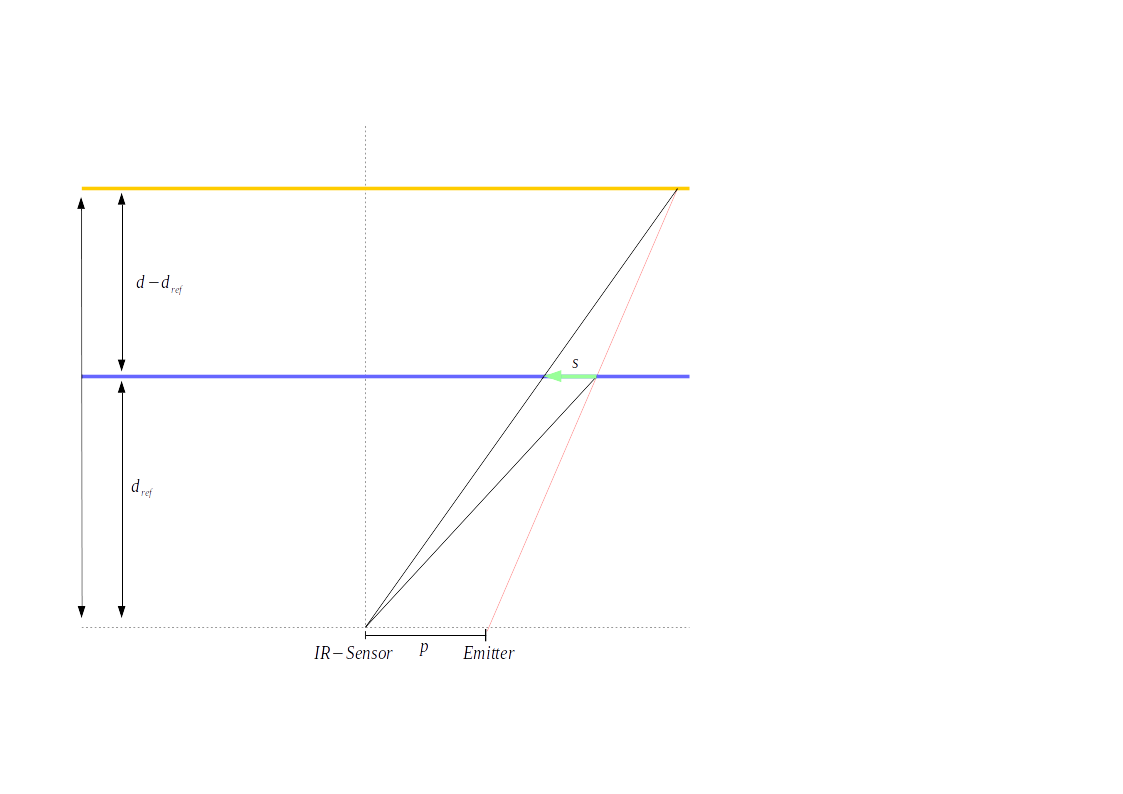
\includegraphics[width=0.8\linewidth]{../media/kinect-depth-principle}
			\caption{}
			\label{fig:kinect-depth-principle}
			\end{figure}
			
			\begin{itemize}
			\item Werte für $d_ref, p$ bekannt
			\item $s$ kann berechnet werden
			\item $\frac{p}{d} = \frac{s}{d-d_ref} \rightarrow d = \frac{p*d_ref}{s-p}$
			\end{itemize}

			
			\subsubsection{Infrarotbilder}
			\subsubsection{Pointclouds}
	\section{OpenCV}
	\section{Robot Operating System}
		\subsection{basics}
		\subsection{Topics \& Nodes}
	\section{Robstep}
	\section{Robotino}